\subsection{Caso d'uso UC8: Apertura di un progetto}
\begin{figure}[h] 
	\centering 
	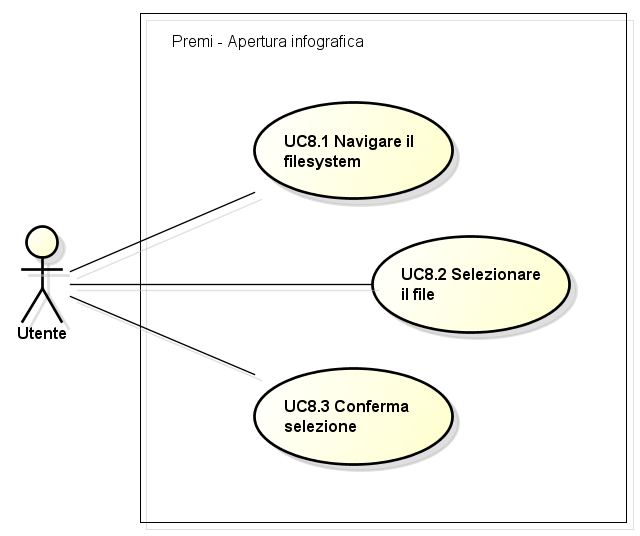
\includegraphics[scale=0.45] {img/UC8.png} 
	\caption{UC8 - Apertura di un progetto} 
\end{figure}

\begin{itemize}
	\item \textbf{Attori:} Proprietario;
	\item \textbf{Scopo e descrizione:} L'utente vuole aprire un progetto esistente;
	\item \textbf{Precondizione:} L'utente ha già creato e salvato un progetto in precedenza;
	\item \textbf{Flusso degli eventi:}
	\begin{enumerate}
		\item L'utente seleziona il progetto da aprire [UC8.1].
	\end{enumerate}
	\item \textbf{Postcondizione:} Il sistema apre la schermata di modifica del progetto.
\end{itemize}


\subsection{Caso d'uso UC8.1: Selezionare il progetto da aprire}
\begin{itemize}
	\item \textbf{Attori:} Proprietario;
	\item \textbf{Scopo e descrizione:} L'utente deve selezionare il progetto che vuole aprire tra quelli selezionati in precedenza;
	\item \textbf{Precondizione:} Il sistema mostra i progetti creati dall'utente;
	\item \textbf{Postcondizione:} Il sistema registra la scelta dell'utente e apre la finestra di modifica.
\end{itemize}

